\documentclass[tikz]{standalone}
\usepackage[dvipsnames,svgnames,x11names]{xcolor}
\usepackage{tikz}
\usepackage{pgfplots}
\usetikzlibrary{pgfplots.statistics}
\pgfplotsset{compat = 1.12}
\usepackage[
  group-separator={,},
  exponent-product=\cdot,
]{siunitx}
\usepackage{../thesismath}
\begin{document}
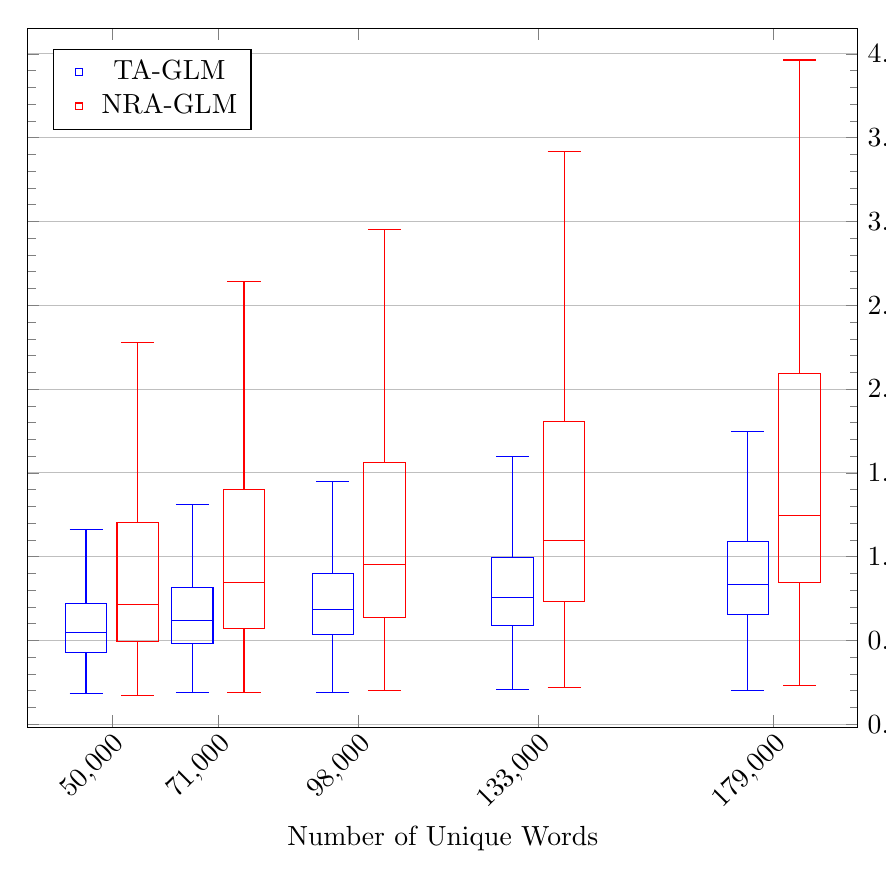
\begin{tikzpicture}[baseline, trim axis left, trim axis right]

\pgfplotscreateplotcyclelist{ta_nra}{%
  blue,  mark size=1.25, mark=square,\\%
  red,   mark size=1.25, mark=square,\\%
}

\pgfplotsset{
  legend style = {
    legend image code/.code = {
      \draw[only marks]
        plot coordinates {
          (0.3cm,0cm)
        };
      \node at (0.15cm, 0cm) {};
      \node at (0.45cm, 0cm) {};
    },
  },
  boxplot/draw/average/.code = {
    % uncomment to show dotted bars for average:
    %\draw[dashed, /pgfplots/boxplot/every average/.try]
    %  (boxplot box cs:\pgfplotsboxplotvalue{average},0)
    %  --
    %  (boxplot box cs:\pgfplotsboxplotvalue{average},1)
    %  ;
  },
}

\sisetup{exponent-base = 2}
\begin{axis}[
%   title = {Calculation Time per top-$1$ Prediction using $5$-grams},
  xlabel = {Number of Unique Words},
  %xtick       = {            1,             2,             3,             4,             5},
  %xticklabels = {\num{1.85e14}, \num{1.85e15}, \num{1.85e16}, \num{1.85e17}, \num{1.85e18}},
  xtick = {50372, 70988, 98209, 133038, 178671},
  xticklabels = {\num{50000}, \num{71000}, \num{98000}, \num{133000}, \num{179000}},
  xticklabel style = {
    inner sep = 1pt,
    anchor = north east,
    rotate = 45,
  },
  ylabel = {Calcluation Time [\si{\milli\second}]},
  yticklabel pos = right,
  ymin = 0.172192,
  ymax = 3.963493,
  scaled x ticks = false,
  scaled y ticks = false,
  minor y tick num = 4,
  y tick label style = {
    /pgf/number format/fixed,
    /pgf/number format/fixed zerofill,
  },
  ymajorgrids = true,
  boxplot/draw direction = y,
  boxplot = {
    box extend = 8000,
  },
  cycle list name = ta_nra,
  enlargelimits = 0.05,
  legend entries = {{TA-GLM}, {NRA-GLM}},
  legend pos = north west,
  width = \textwidth,
]

% ------------------------------------------------------------------------------

% training-5-argmaxcompare-40k-c/ngram-5-TA-Weighted-Sum-Generalized-Language-Model-1
\addplot+[
  boxplot prepared = {
    draw position = 45372,
    lower whisker = 0.182297,
    lower quartile = 0.427452,
    median = 0.545453,
    upper quartile = 0.720338,
    upper whisker = 1.159506,
    average = 0.614068,
  },
] table [row sep = \\, y index = 0] {
  data\\
};

% training-5-argmaxcompare-40k-c/ngram-5-NRA-Weighted-Sum-Generalized-Language-Model-1
\addplot+[
  boxplot prepared = {
    draw position = 55372,
    lower whisker = 0.172192,
    lower quartile = 0.492755,
    median = 0.714188,
    upper quartile = 1.206376,
    upper whisker = 2.276287,
    average = 1.227375,
  },
] table [row sep = \\, y index = 0] {
  data\\
};

% ------------------------------------------------------------------------------

% training-4-argmaxcompare-40k-c/ngram-5-TA-Weighted-Sum-Generalized-Language-Model-1
\addplot+[
  boxplot prepared = {
    draw position = 65988,
    lower whisker = 0.189782,
    lower quartile = 0.483218,
    median = 0.617765,
    upper quartile = 0.813524,
    upper whisker = 1.308804,
    average = 0.692814,
  },
] table [row sep = \\, y index = 0] {
  data\\
};

% training-4-argmaxcompare-40k-c/ngram-5-NRA-Weighted-Sum-Generalized-Language-Model-1
\addplot+[
  boxplot prepared = {
    draw position = 75988,
    lower whisker = 0.191494,
    lower quartile = 0.571501,
    median = 0.845661,
    upper quartile = 1.399696,
    upper whisker = 2.641562,
    average = 1.422414,
  },
] table [row sep = \\, y index = 0] {
  data\\
};

% ------------------------------------------------------------------------------

% training-3-argmaxcompare-40k-c/ngram-5-TA-Weighted-Sum-Generalized-Language-Model-1
\addplot+[
  boxplot prepared = {
    draw position = 93209,
    lower whisker = 0.187163,
    lower quartile = 0.535744,
    median = 0.685056,
    upper quartile = 0.899978,
    upper whisker = 1.446284,
    average = 0.771727,
  },
] table [row sep = \\, y index = 0] {
  data\\
};

% training-3-argmaxcompare-40k-c/ngram-5-NRA-Weighted-Sum-Generalized-Language-Model-1
\addplot+[
  boxplot prepared = {
    draw position = 103209,
    lower whisker = 0.200491,
    lower quartile = 0.636782,
    median = 0.951191,
    upper quartile = 1.564153,
    upper whisker = 2.954344,
    average = 1.641707,
  },
] table [row sep = \\, y index = 0] {
  data\\
};

% ------------------------------------------------------------------------------

% training-2-argmaxcompare-40k-c/ngram-5-TA-Weighted-Sum-Generalized-Language-Model-1
\addplot+[
  boxplot prepared = {
    draw position = 128038,
    lower whisker = 0.207189,
    lower quartile = 0.591446,
    median = 0.755523,
    upper quartile = 0.994264,
    upper whisker = 1.598150,
    average = 0.855940,
  },
] table [row sep = \\, y index = 0] {
  data\\
};

% training-2-argmaxcompare-40k-c/ngram-5-NRA-Weighted-Sum-Generalized-Language-Model-1
\addplot+[
  boxplot prepared = {
    draw position = 138038,
    lower whisker = 0.219336,
    lower quartile = 0.731608,
    median = 1.094962,
    upper quartile = 1.806765,
    upper whisker = 3.418836,
    average = 1.912399,
  },
] table [row sep = \\, y index = 0] {
  data\\
};

% ------------------------------------------------------------------------------

% training-1-argmaxcompare-40k-c/ngram-5-TA-Weighted-Sum-Generalized-Language-Model-1
\addplot+[
  boxplot prepared = {
    draw position = 173671,
    lower whisker = 0.202749,
    lower quartile = 0.654436,
    median = 0.832421,
    upper quartile = 1.092418,
    upper whisker = 1.749261,
    average = 0.952469,
  },
] table [row sep = \\, y index = 0] {
  data\\
};

% training-1-argmaxcompare-40k-c/ngram-5-NRA-Weighted-Sum-Generalized-Language-Model-1
\addplot+[
  boxplot prepared = {
    draw position = 183671,
    lower whisker = 0.233460,
    lower quartile = 0.843436,
    median = 1.245531,
    upper quartile = 2.091483,
    upper whisker = 3.963493,
    average = 2.339178,
  },
] table [row sep = \\, y index = 0] {
  data\\
};

\end{axis}

\end{tikzpicture}
\end{document}
